\newpage
\subsubsection{BLDC}
\label{subsubsec:BLDC}

Ein BLDC zeichnet sich dadurch aus, dass der Rotor mit Permanentmagneten bestückt ist. Somit ähnelt er vom Aufbau her einer Synchronmaschine mit permanenterregten Rotorwicklungen. Zur Ansteuerung hat der BLDC drei Phasenleitungen, welche auf die Spulen führen. Die Spulen sind innerhalb des BLDC in Stern geschaltet. Der Motor hat drei Polpaare, womit die magnetische Winkelgeschwindigkeit drei Mal schneller ist als die mechanische.

Ein Nachteil von BLDC-Motoren ist, dass bei Drehgeschwindigkeiten über Nenndrehzahl nur mit einer geeigneten Regelung der Statorwicklungen in Feldschwächung gefahren werden kann, anstelle dass der Erregerstrom verringert wird. Ansonsten zeichnet sich ein BLDC durch ein besseres Leistungs-/Gewichtsverhältnis aus als herkömmliche Motoren.

\paragraph{Schaltungsaufbau}\mbox{}

Der Motor wird direkt auf die vorgesehenen Anschluss-Pins geführt. Obwohl die Versorgungsspannung unterhalb der maximalen Berührungsspannung liegt wurde im Falle eines Defekts im Motor zur Personensicherheit ein Pin für die Erdung des Motorengehäuses vorgesehen.

\begin{figure}[h!]
	\centering
	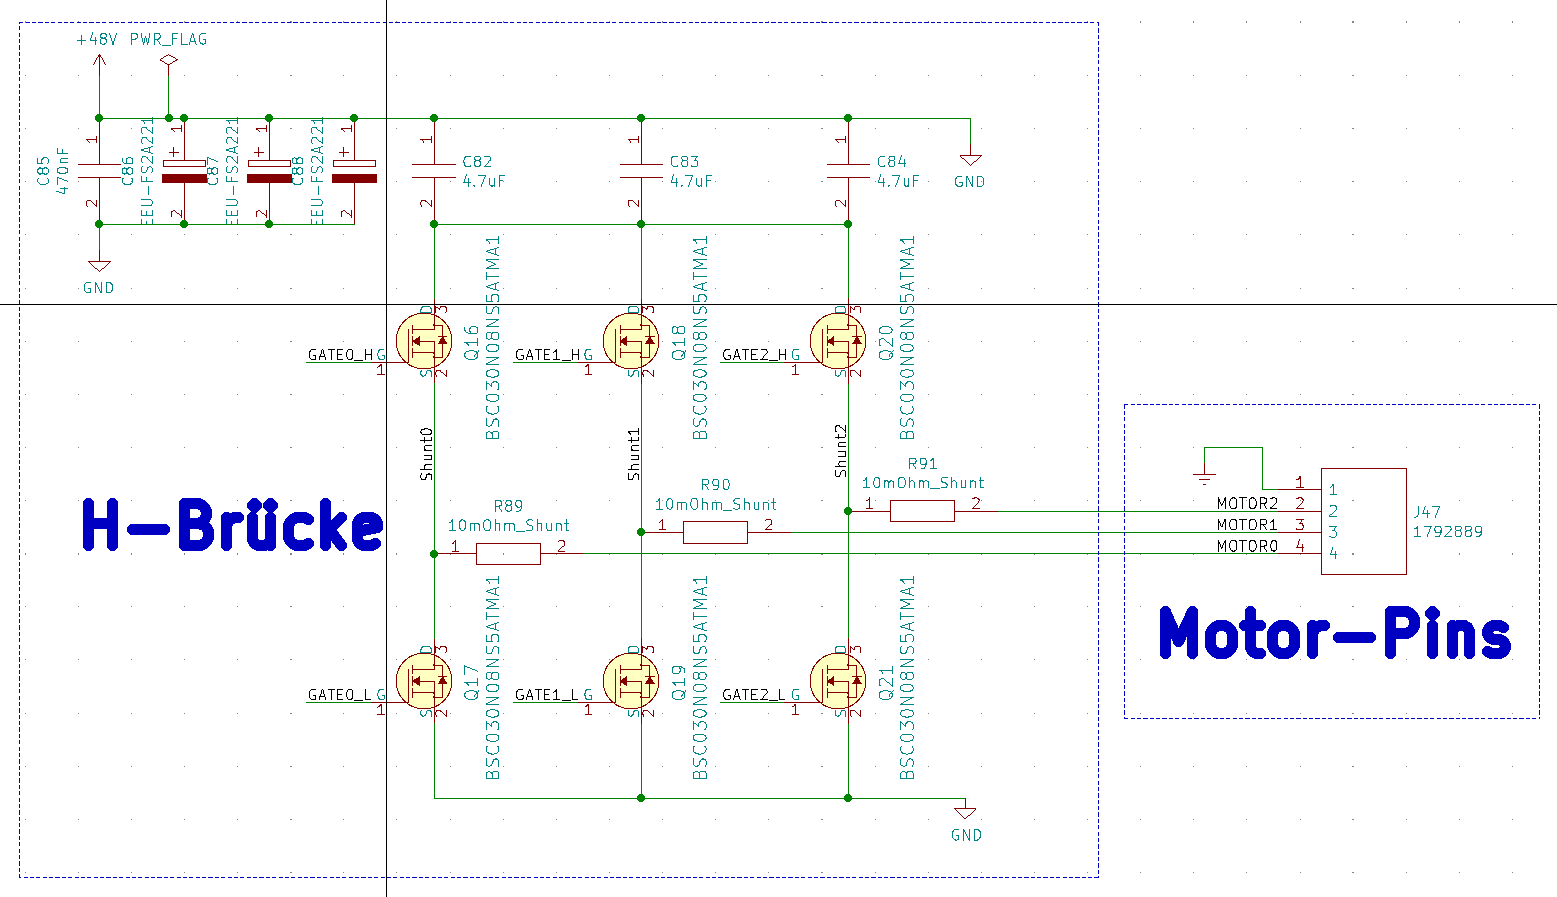
\includegraphics[width=0.5\textwidth]{graphics/Schema_H_Bruecke_und_BLDC}
	\caption{H-Brücke und Motor-Pins für BLDC}
	\label{fig:Schema_H_Bruecke_und_BLDC}
\end{figure}

\paragraph{Funktionsbeschrieb der Schaltung}\mbox{}

Hier gibt es nicht viel zu beschreiben, der Anschluss des Motors ist selbsterklärend. Lediglich die Phasenfolge ist zu beachten, damit das Drehfeld stimmt.

Der Motor an sich lässt sich wie folgt beschreiben:

\begin{tabular}{lllll}
Nennnetzspannung & $V_M$ & = & 48 & [V]\\
Stillstanddrehmoment & $M_0$ & = & 0.88 & [Nm]\\
Nenndrehmoment & $M_n$ & = & 0.85 & [Nm]\\
Spitzendrehmoment & $M_{0max}$ & = & 2.8 & [Nm]\\
Nenndrehzahl & $n_n$ & = & 1500 & [min$^{-1}$]\\
Nennleistung & $P_n$ & = & 0.13 & [kW]\\
Stillstandstrom & $I_0$ & = & 5.41 & [A]\\
Nennstrom & $I_N$ & = & 5.21 & [A]\\
Spitzenstrom & $I_{max}$ & = & 21.6 & [A]\\
Drehmomentkonstante & $k_T$ & = & 0.1632 & [Nm/A]\\
Rotorträgheitsmoment & $J$ & = & 0.16 & [kg$\cdot$cm$^2$]\\
Gewicht & $m$ & = & 1.1 & [kg]\\
\end{tabular}